\documentclass[a4paper, 12pt, twoside]{article}
\usepackage{cmap} % Улучшенный поиск русских слов в полученном pdf-файле
\usepackage[T2A,T1]{fontenc}
\usepackage[utf8]{inputenc}
\usepackage[english, russian]{babel}
\usepackage{graphicx}
\usepackage[hcentering, bindingoffset = 10mm, right = 15 mm, left = 15 mm, top=20mm, bottom = 20 mm]{geometry}
\usepackage{multirow}
\usepackage{lipsum}
\usepackage{amsmath, amstext}
\usepackage{siunitx}
\usepackage{subcaption}
\usepackage{wrapfig}
\usepackage{adjustbox}
\usepackage{enumerate, indentfirst, float}
\usepackage{capt-of, svg}
\usepackage{ctable}


\usepackage{pscyr} % Нормальные шрифты
\usepackage[normalem]{ulem} % для подчёркиваний uline
\ULdepth = 0.16em

\usepackage{fancyhdr} %Колонтикулы
\pagestyle{fancy}
\lhead{
\includegraphics[width = 10 mm]{logo.jpg} Лабораторная работа № 3.4.2}
\rhead{\textit{\today}}

\newenvironment{bottompar}{\par\vspace*{\fill}}{\clearpage}
 
\begin{document}
\begin{titlepage}

\newcommand{\HRule}{\rule{\linewidth}{0.7mm}} % Defines a new command for the horizontal lines, change thickness here

\center % Center everything on the page
 
%----------------------------------------------------------------------------------------
%	HEADING SECTIONS
%----------------------------------------------------------------------------------------

\textsc{\LARGE Московский Физико-Технический Институт}\\[1,5cm] % Name of your university/college
\textsc{\Large Кафедра общей физики}\\[0.5cm] % Major heading such as course name
\textsc{\large Лабораторная работа \textnumero  3.4.2}\\[0.5cm] % Minor heading such as course title

%----------------------------------------------------------------------------------------
%	TITLE SECTION
%----------------------------------------------------------------------------------------

\HRule
\\[0.4cm]
{ \huge \bfseries Закон Кюри-Вейса.}
\\[0.2cm] % Title of your document
\HRule
\\[1.5cm]


 
%----------------------------------------------------------------------------------------
%	AUTHOR SECTION
%----------------------------------------------------------------------------------------

\begin{minipage}{0.4\textwidth}
	\begin{flushleft} \large
		\textbf{Автор:}\\
		Глеб Уваркин \\
		615 группа
	\end{flushleft}
\end{minipage}
~
\begin{minipage}{0.4\textwidth}
	\begin{flushright} \large
		\textbf {Преподаватель:} \\
		Андрей Александрович Заболотных % Supervisor's Name
	\end{flushright}
\end{minipage}

\begin{bottompar}
	\begin{center}
		
\includegraphics[width = 80 mm]{logo.jpg}
	\end{center}
	{\large \today}

\end{bottompar}
\vfill % Fill the rest of the page with whitespace

\end{titlepage}

{\Large \uline { \textbf  {Цель работы:}}}

\vspace{2mm}
Изучение температурной зависимости магнитной восприимчивости ферромагнетика выше точки Кюри.
\vspace{\baselineskip}

{\Large \uline { \textbf  {В работе используются:}}}

\vspace{2mm}

Катушка самоиндукции с образцом из гадолиния, термостат, частотометр, цифровой вольтметр, LC-автогенератор, термопара медь-константан.

\section{Теоретические сведения.}
Внешнее магнитное поле ориентирует магнитные моменты, которые в отсутствии поля располагались в пространстве хаотичным образом.
При повышении температуры $T$ возрастает дезориентирующее действие теплового движения частиц, и магнитная восприимчивость парамагнетиков убывает, в простейшем случае (в постоянном магнитном поле) - по закону Кюри: 
\begin{equation}
\chi = \dfrac{C}{T}, \label{eq1}
\end{equation}
где С - постоянная Кюри.

Для парамагнитных веществ, которые при понижении температуры становятся ферромагнитными формула \eqref{eq1} должна быть видоизменена. Эта формула показывает, что температура $T=0$ является особой точкой температурной кривой, в которой $\chi$ неограничено возрастает.

При $T\rightarrow 0$ тепловое движение все меньше препятствует магнитным моментам атомов ориентироваться в одном направлении при сколь угодно слабом внешнем поле. В ферромагнетиках -  под влиянием обменных сил -  это происходит при понижении температуры не до абсолютного нуля, а до температуры Кюри $\Theta$. Оказывается, что у ферромагнетиков закон Кюри должен быть заменен законом Кюри-Вейсса:
\begin{equation}
\chi \sim \dfrac{1}{T-\Theta_p} ,
\label{eq2}
\end{equation}
где $\Theta_p$- температура, близкая к температуре Кюри. 

Эта формула хорошо описывает поведение ферромагнитных веществ после их перехода в парамагнитную фазу при заметном удалении температуры от $\chi$, но недостаточна точна при $T \approx \chi$.

В нашей работе мы изучаем температурную зависимость $\chi(T)$ гадолиния при температурах выше точки Кюри. Для гадолиния точка Кюри лежит в пределах комнатных температур.

\begin{figure}[H]
	\centering
	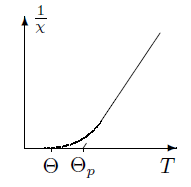
\includegraphics[width = 0.25 \textwidth]{shema1.png}
	\caption{Зависимость обратной величины магнитной восприимчивости от температуры}
\end{figure}
\section{Экспериментальная установка.}

\begin{figure}[H]
	\centering
	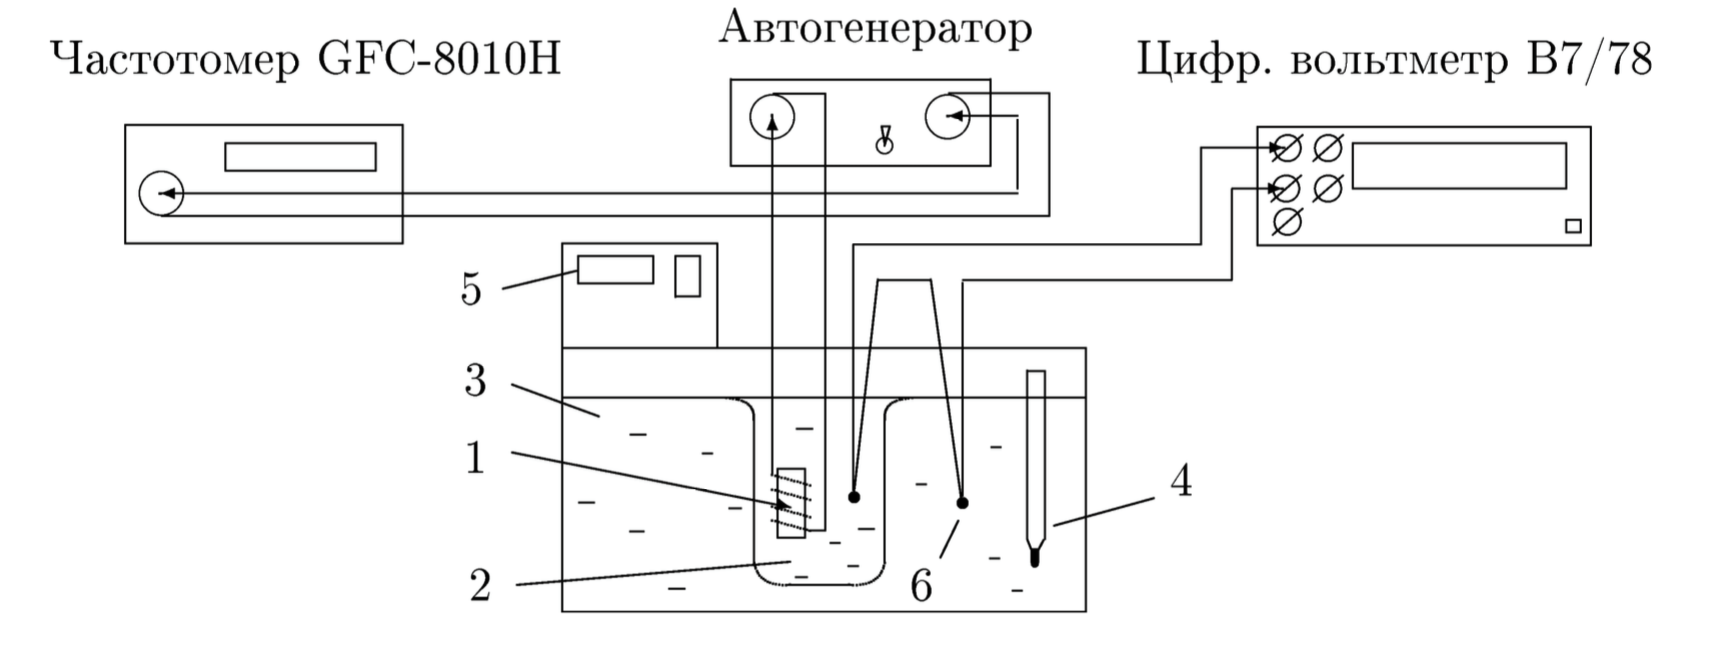
\includegraphics[width = 0.8 \textwidth]{shema2}
	\caption{Схема экспериментальной установки}
	
	\textit{1 - Катушка с образцом, 2 - стеклянный сосуд с трансформаторным маслом, 3 - вода в термостате, 4 - ртутный термометр, 5 - термостат}
\end{figure}

Гадолиний является хорошим проводником электрического тока, а рабочая частота генератора достаточно велика ($\sim$50кГц), поэтому для уменьшения вихревых токов образец изготовлен из мелких кусочков размером около 0,5 мм. Катушка 1 с образцом помещена в стеклянный сосуд 2, залитый трансформаторным маслом. Масло предохраняет образец от окисления и способствует ухудшению электрического контакта между отдельными частичками образца. Кроме того, оно улучшает тепловой контакт между образцом и термостатируемой (рабочей) жидкостью 3 в термостате. Ртутный термометр 4 используется для приближенной оценки температуры. Температура образца регуляруется с помощью термостата.

Магнитная восприимчивость образца $\chi$ определяется по изменению самоиндукции катушки. Обозначив через $L$ самоиндукцию катушки с образцом и через $L_0$ - её самоиндукцию в отсутствии образца, получим 

\begin{equation}
(L-L_0) \sim \chi.
\label{eq3}
\end{equation}

При изменении самоиндукции образца меняется период колебаний автогенератора:

\begin{equation}
\tau = 2\pi\sqrt{LC} ,
\label{eq4}
\end{equation}
где $C$ - ёмкость контура автогенератора.

Период колебаний в отсутствие образца определяется самоиндукцией пустой катушки:

\begin{equation}
\tau_0 = 2\pi\sqrt{L_0C} ,
\label{eq5}
\end{equation}

Из \eqref{eq4} и \eqref{eq5} имеем

$$ (L-L_0) \sim (\tau^{2}-\tau_0^{2}). $$

Таким образом,

\begin{equation}
\chi \sim (\tau^{2}-\tau_0^{2}).
\label{eq6}
\end{equation}

Из формул \eqref{eq2} и \eqref{eq6} следует, что закон Кюри-Вейсса справедлив, если выполнено соотношение 

\begin{equation}
\dfrac{1}{\chi} \sim (T- \Theta_p) \sim \dfrac{1}{(\tau^2-\tau_0^2)}.
\label{eq7}
\end{equation}

\textbf{Параметры установки:} $k = 24 ~\text{град/мВ}$ ,
$\tau_0 = 6,95636 \text{мкс}$.


\section{Обработка результатов.}
Нашей задачей является проверка выполнения закона Кюри-Вейса. Зная, что при изменении температуры должна меняться магнитная восприимчивость гадолиния, а, следовательно, и самоиндукция катушка, будем замерять период колебания $\tau$ в колебательном контуре в зависимости от температуры вещества $T$. Разность между температурой в термостате $T_\text{изм.}$ и реальной температурой вещества можно оценить с помощью термопары $\Delta U$ и коэффициента установки $k$. Проверим выполнение соотношения \eqref{eq7}.

\begin{table}[H]
	\centering
	\resizebox{\textwidth}{!}{%
		\begin{tabular}{c|ccccccccccccc}
			\toprule
			$T_\text{изм.}, \SI{}{\degreeCelsius}$    & 16.000 & 18.100 & 20.100 & 22.100 & 24.100 & 26.060 & 28.050 & 30.050 & 32.000 & 34.000 & 36.000 & 38.000 & 40.000  \\ 
			$\Delta U, \text{мВ}$        & -0.003  & -0.020 & -0.020 & -0.020 & -0.013 & -0.015 & -0.018 & -0.016 & -0.015 & -0.010 & 0 & 0,010 & 0,010 \\ 
			$T, \SI{}{\degreeCelsius}$       & 15.928 & 17.620 & 19.620 & 21.620 & 23.788 & 25.700 & 27.618 & 29.666 & 31.640 & 34.240 & 36.000 & 38.240 & 40.240 \\ 
			$\tau, \text{мкс}$    & 7.880  & 7.770  & 7.590  & 7.390  & 7.210  & 7.130  & 7.090  & 7.060  & 7.040  & 7.030  & 7.018  & 7.009  & 7.003    \\ 
			$\tau^2 -\tau_0^2, \text{мкс}^2 $     & 13.703 & 11.982 & 9.217 & 6.221 & 3.593  & 2.446  &  1.877 & 1.453  & 1.171  & 1,029  & 0.861  & 0.735  & 0.651   \\ 
			$1/(\tau^2 -\tau_0^2), 1/\text{мкс}^2 $  & 0.073  & 0.083  & 0.108  & 0.161  & 0.278  & 0.409  & 0.533  & 0.688  & 0.854  & 0.971  & 1.161  & 1.360  & 1.536   \\ \midrule
			$\Delta T, \SI{}{\degreeCelsius}$&0.010&0.881&0.981&1.081&1.829&1.713&1.534&1.854&2.109&3.424&0.010&3.824&4.024 \\
		  \bottomrule
		\end{tabular}%
	}
	\caption{Данные с установки}
\end{table}

Построим график зависимости $\tau^2-\tau_0^2 = f(T)$.
\begin{figure}[H]
	\centering
	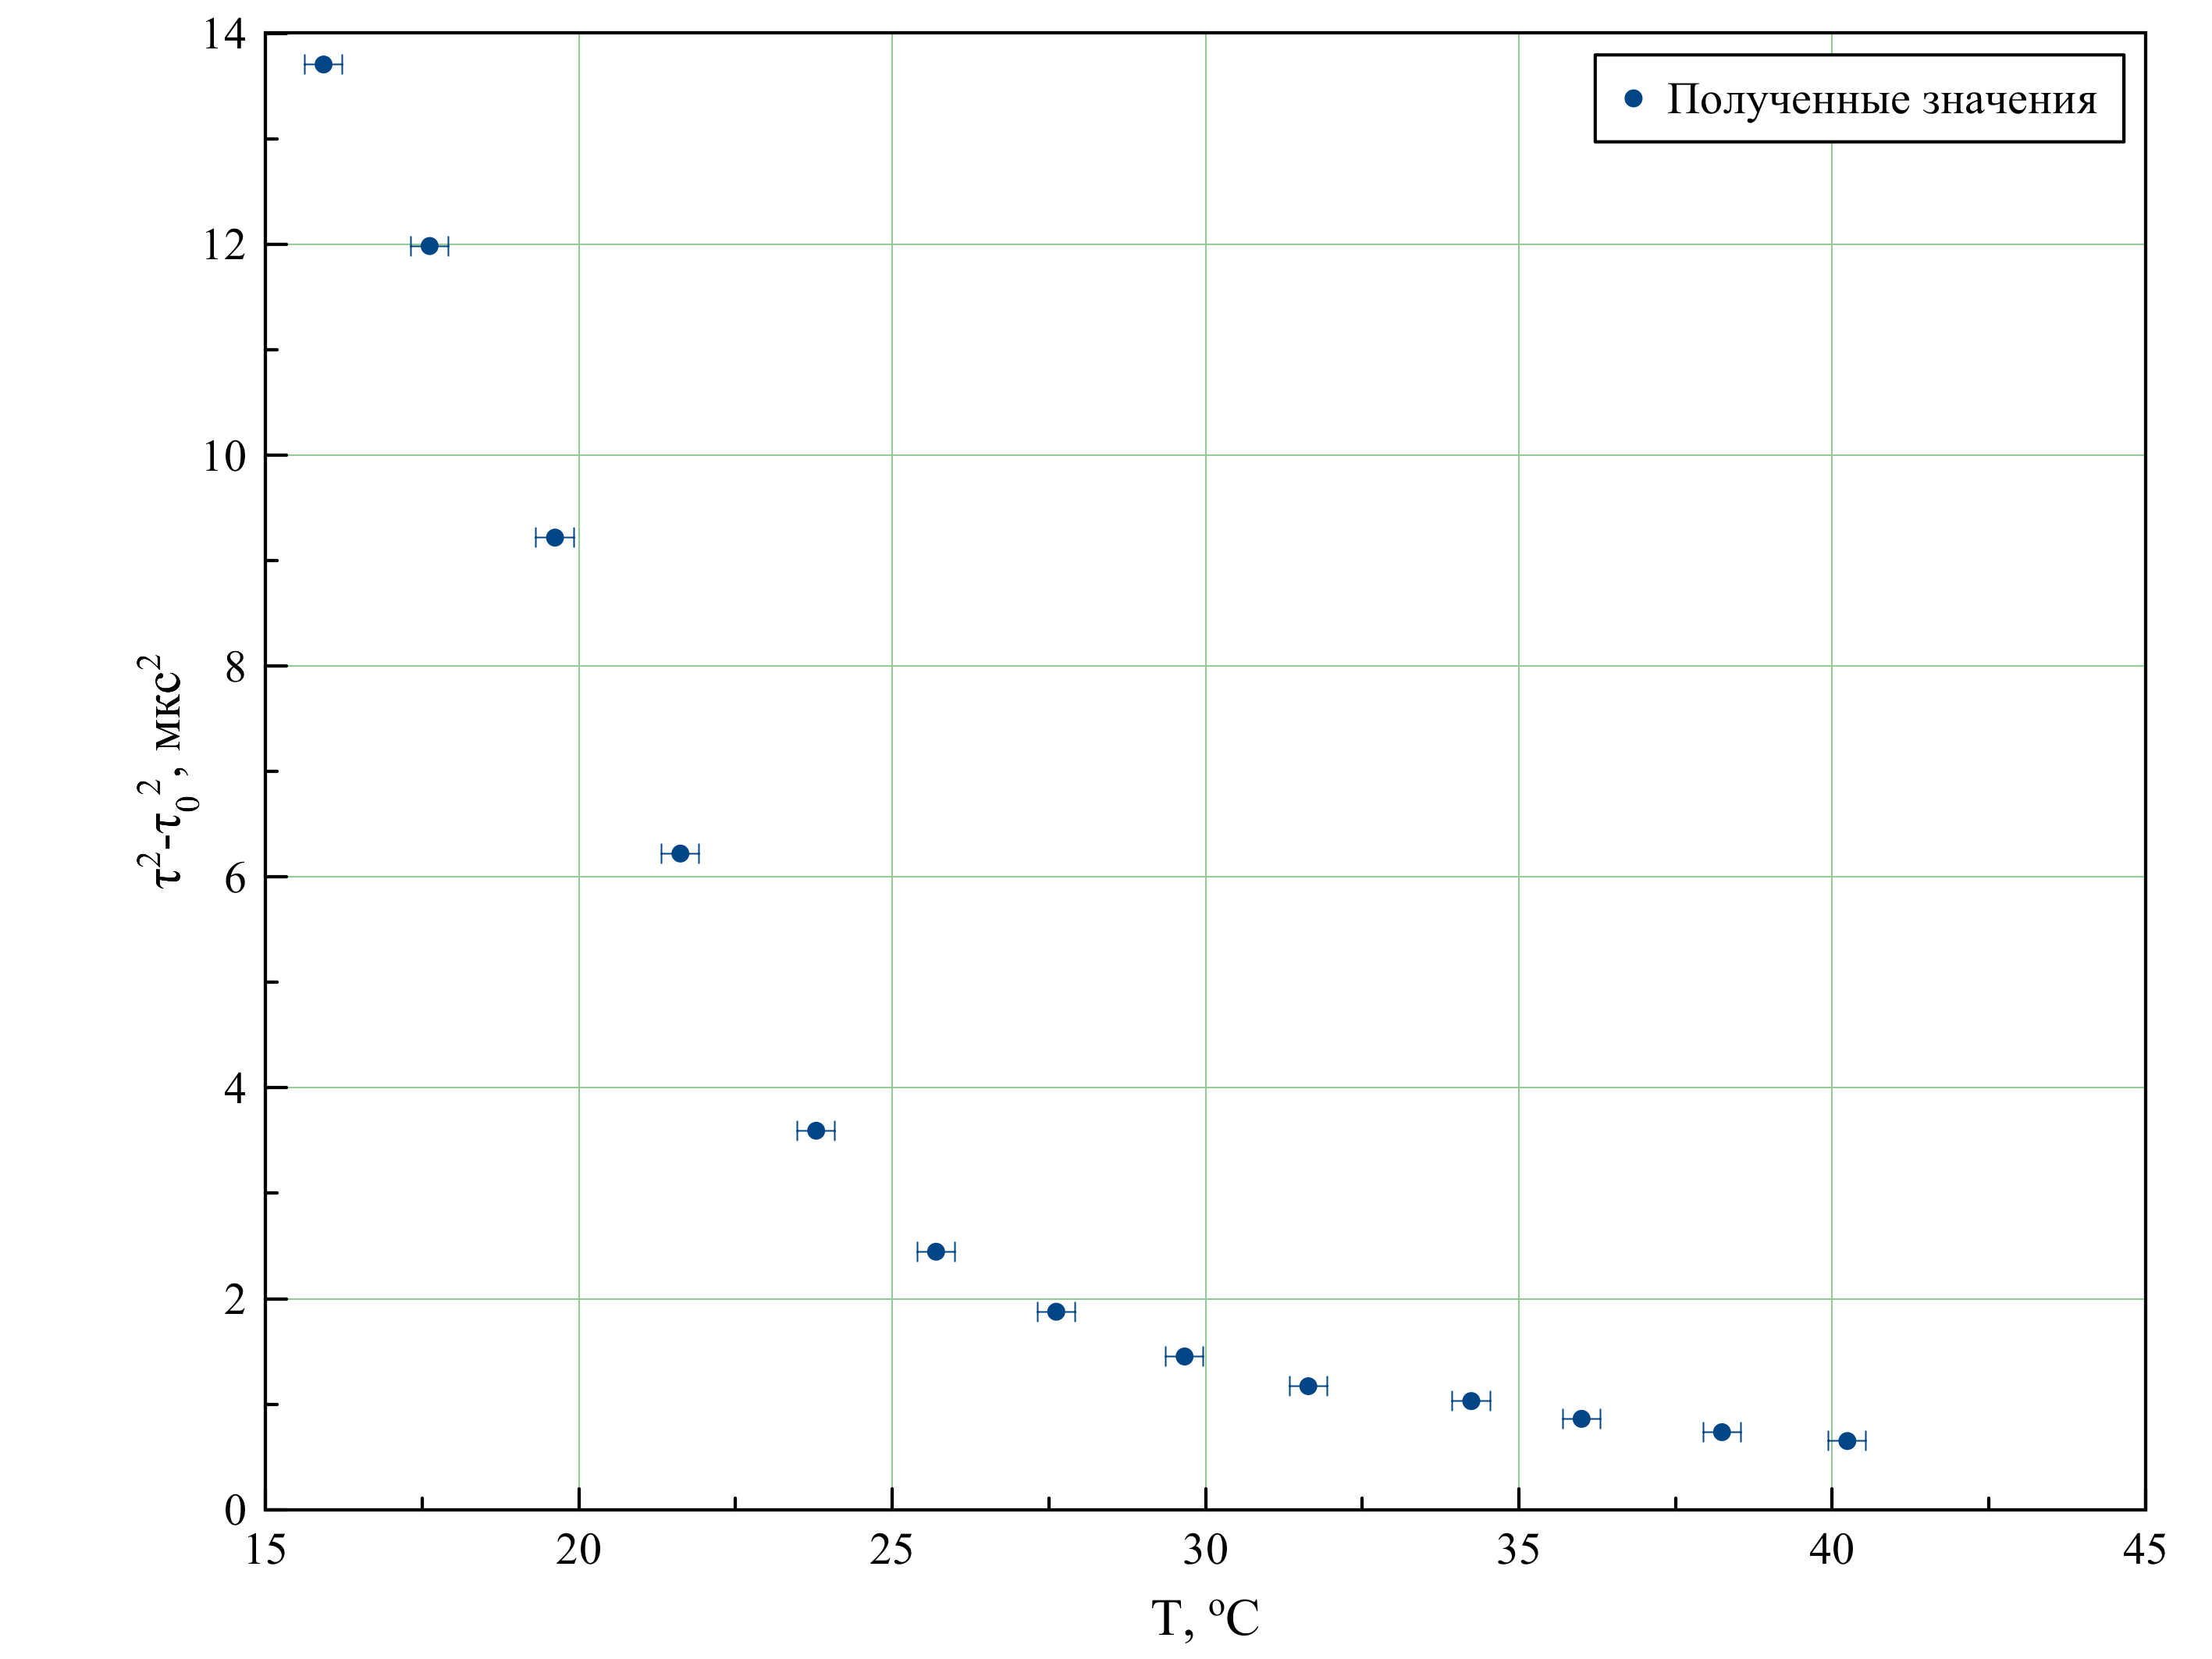
\includegraphics[width = 0.8 \textwidth]{1}
	\caption{График зависимости $\tau^2-\tau_0^2 = f(T)$.}
\end{figure}

По данному графику сложно определить температуру Кюри, так как было снято слишком мало точек при низкой температуре (установка позволила провести измерения лишь при температуре $ >16\SI{}{\degreeCelsius}$. )

\begin{figure}[H]
	\centering
	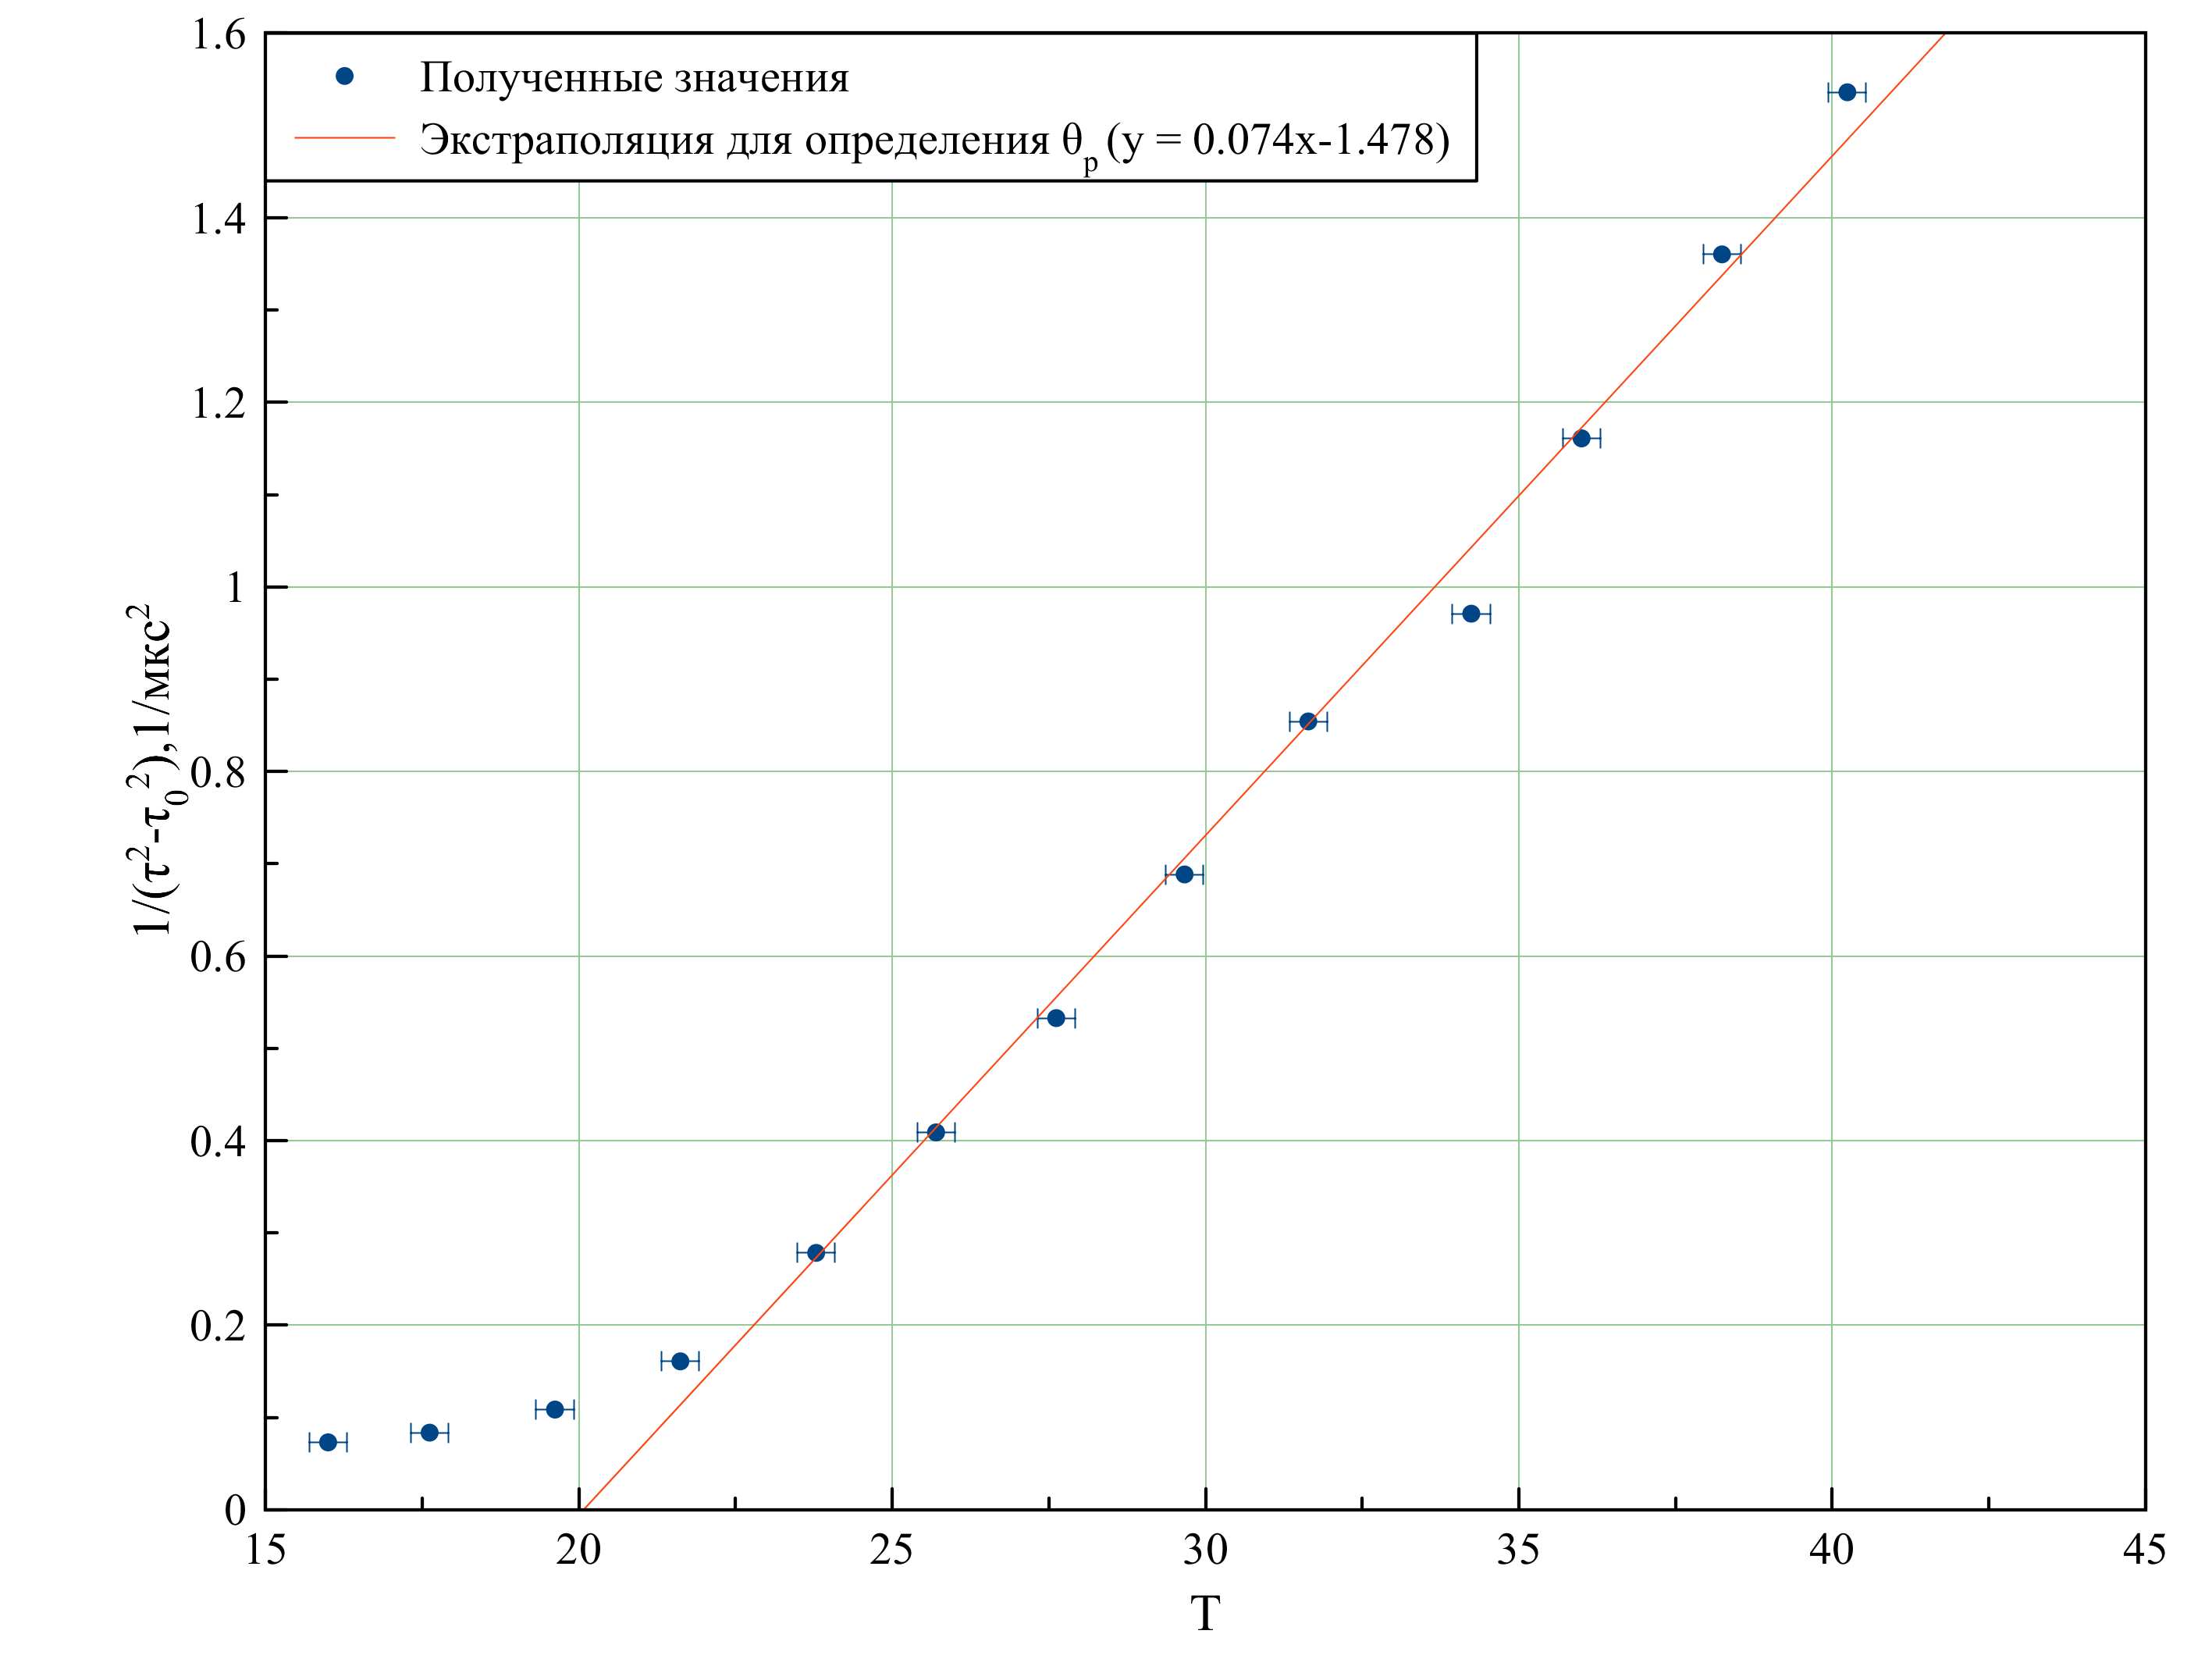
\includegraphics[width = 0.8 \textwidth]{2}
	\caption{График зависимости $1/(\tau^2-\tau_0^2) = f(T)$.}
\end{figure}

С помощью метода наименьших квадратов определим значение $\Theta_p$ и её погрешность:
\begin{equation*}
\fbox{\text{$\Theta_p \simeq (19.97 \pm 0.51) ~ \SI{}{\degreeCelsius}$} ($\varepsilon \simeq 3 \%$)}
\end{equation*}

Табличное значение парамагнитной температуры Кюри для гадолиния $\Theta_p = 16 \SI{}{\degreeCelsius}. $

\section{Вывод.}
Полученное значение температуры Кюри близко к табличному, но все же не совпадает с ним. Причиной этому могла послужить неисправность установки, неточность измерений, вызванная разницей температур установки и образца, а также небольшое количество измерений в окрестности точки Кюри.


\end{document}
